\documentclass{article}
\usepackage[a4paper, margin=2cm]{geometry}

\usepackage{amsmath}
\usepackage{amssymb}
\usepackage{mathtools}
\usepackage{amstext}
\usepackage{amsthm}
\usepackage{fancyhdr}
\usepackage{siunitx}

\usepackage{hyperref}


\usepackage{quoting}

\usepackage{graphicx}
\usepackage{booktabs}
\graphicspath{{figures/}} %Setting the graphicspath
\usepackage{float}
\usepackage{caption}
\usepackage{subcaption}

% To work with inkfigures
\usepackage{import}
\usepackage{pdfpages}
\usepackage{transparent}
\usepackage{xcolor}

\newcommand{\incfig}[2][1]{%
    \def\svgwidth{#1\columnwidth}
    \import{./figures/}{#2.pdf_tex}
}

\pdfsuppresswarningpagegroup=1

%\graphicspath{{figures/}}

\pagestyle{fancy}
\rhead{Alexandre Adam}
\lhead{PHY6669 - Cosmologie \\ Alan Robinson}
\chead{}
\rfoot{\today}
\cfoot{\thepage}

\newcommand{\angstrom}{\textup{\AA}}
\numberwithin{equation}{section}
\renewcommand\thesubsection{\alph{subsection})}
\renewcommand\thesubsubsection{\roman{subsubsection})}
\newcommand{\s}{\hspace{0.1cm}}

%\usepackage[backend=bibtex,bibencoding=ascii,style=authoryear,sorting=none]{biblatex}
%\usepackage{biblatex}
%\addbibresource{bibfile.bib}

\newcommand{\pyoutput}[2]{#2}

\DeclareSIUnit\parsec{pc}

\begin{document}

\section{Le paradoxe d'Olber}
Le paradoxe d'Olber peut être déclaré de la façon suivante: 
\begin{quoting}
        Dans un univers infinie populé de façon homogène par des étoiles, le ciel serait 
        au moins aussi brillant que le Soleil.
\end{quoting}
En effet, supposant une densité cosmique constante $n_\star$ et une luminosité moyenne $L_\star$, 
alors le flux reçu (erg $\angstrom^{-1}$ cm$^{-2}$ s$^{-1}$) serait 
\[
        \frac{d I}{d \Omega} \sim \int_0^\ell n_\star \frac{L_\star}{r^2} r^2 dr 
        = n_\star \ell L_\star  = \frac{L_\star}{\pi R_\star^2}
\]
pour $\ell$ définit comme le libre parcours moyen d'un photon dans cet univers.
La cosmologie moderne résout ce paradoxe en introduisant un âge finit à l'Univers ainsi 
qu'une expansion, ce qui crée un horizon cosmique.
\subsection{Énoncé}

Dans ces cosmologies, quel serait donc le redshift median auquel on s'attend lorsqu'on 
compile une large population de galaxies et d'étoiles? Notre stratégie pour évaluer cette 
quantité est fondée sur l'idée que le redshift médian correspond à 
\[
        \left( \frac{\partial I_{\lambda_0}}{\partial \Omega} \right)_{\max}^{-1} 
        \frac{\partial I_{\lambda_0}}{\partial \Omega}(z_{\text{median}}) = 0.5
\]
où la médiane est définit relativement à une distribution cumulative du flux radiatif.
Un équivalent bolométrique peut aussi être 
calculé. En d'autre mots, le redshift médian correspond au temps (passé)
à partir duquel la moitié des photons 
nous provenant des galaxies et des étoiles ont été émis.

\subsection{Dérivation}
La métrique FRW est définit avec l'observateur $\mathcal{O}$ 
situé à l'origine du système de coordonées. Une section du 
volume d'une coquille entre la coordonnée comobile $r$ et $r + dr$ est
\[
        \frac{\partial V_{\text{coquille}} }{\partial \Omega}= 
        %\int_{\theta=0}^{\pi} \int_{\phi=0}^{2\pi} 
        \frac{a dr}{\sqrt{1 - kr^2}}
        a^2r^2 %\sin \theta d\theta d\phi 
        %= \frac{4 \pi a^3 r^2dr}{\sqrt{1 - kr^2}}
\]
Pour une cosmologie de poussière (dominée par la matière $\implies p = 0$), 
la conservation de l'entropie impose que la densité varie selon 
\[
        \rho \propto a^{-3 }
\]
Dans ce cas, la densité numérique des étoiles et galaxies varie selon
\[
        n(t) = n_0 \left( \frac{a_0}{a(t)} \right)^3
\]
On définit le flux spécifique $f_\lambda(t)$ 
à partir de la fonction de Planck (ce qui est une approximation du spectre 
produit par une collection de galaxies)
\begin{equation}\label{eq:flux} 
        f_\lambda(t)d\lambda \equiv C(t) \frac{4 \pi \hbar c^2}{\lambda^5 } 
        \frac{d\lambda}{\exp \left\{\dfrac{ 2 \pi \hbar c }{k_bT \lambda}\right\} -1 }
\end{equation} 
où $C$ est un constante qui peut en principe dépendre du temps pour refléter l'évolution des 
galaxies et des étoiles. Notons que la température peut elle aussi dépendre du temps pour 
refléter les cycles d'évolution des étoiles.
%Une galaxie à l'intérieur de la coquille qui émet dans 
%la bande d'onde $\lambda$ à $\lambda + d\lambda$ va émettre un flux de photon observé à 
%$\mathcal{O}$ avec une une longueur d'onde $\lambda_0 = \lambda(1 + z)$. 
La contribution des 
galaxies se situant dans la coquille mesurée par l'observateur produit une intensité
\[
        d(\frac{\partial I_\lambda}{\partial \Omega}) d\lambda
        = \frac{\partial V_{\text{coquille}} }{\partial \Omega}n(t)\frac{f_\lambda(t) }{4 \pi a_0^2r^2(1 + z)^2}d\lambda
\]
Notons que les photons produits dans un interval de temps
$\delta $ arrive à l'observateur dans un interval de temps  
$\delta_0 = \delta (1 + z)$ selon l'effet de dilatation temporelle. Le second facteur de redshift 
vient du fait que l'énergie du photon est proportionnel à $E_\lambda = ch/\lambda$. L'énergie 
de chaque photon est réduit: $E_{\lambda_0}= ch/\lambda(1 + z)$
%où la puissance 2 au facteur $(1 + z)$ vient de la contribution de l'expansion de l'univers mais 
%aussi du fait qu'un photon émit avec une longueur d'onde $\lambda$ est observé 
%avec une longueur d'onde $\lambda_0 = \lambda(1 + z)$.

Il est pratique de travailler avec la coordonnée $cdt$ plutôt que la coordonnée radiale $dr$ 
sachant que les photons suivent une géodésique radial
\[
        cdt = \frac{adr}{\sqrt{1 - kr^2}}
\]
De sortes que 
\[
        d(\frac{\partial I_\lambda}{\partial \Omega}) 
        d\lambda= \frac{cn_0 }{4 \pi}f_\lambda(t) \frac{a(t)}{a_0} dtd\lambda 
\]
Pour connecter avec les observations, on doit exprimer cette quantité en terme de $\lambda_0$ 
ce qui fait apparaître un facteur de redshift supplémentaire:
\begin{equation}\label{eq:intensity} 
        d(\frac{\partial I_{\lambda_0}}{\partial \Omega}) d\lambda_0 = 
        \frac{c n_0}{4 \pi} f_{\lambda_0}(t) 
        \left( \frac{a(t)}{a_0} \right)^{2}d\lambda_0 dt
\end{equation} 
%et la luminosité [olométrique des galaxies ayant émis au temps $t$ est 
%\begin{equation}\label{eq:Lbol} 
        %L(t) \equiv \int_0^\infty f_\lambda(t)d\lambda %= \frac{C\sigma_{\text{SB}}}{\pi}T^4
%\end{equation} 
L'intensité spécifique reçut par $\mathcal{O}$ est donc 
\begin{equation}\label{eq:Ispec} 
        \frac{\partial I_{\lambda_0}}{\partial \Omega} = 
        \frac{cn_0}{4 \pi}
        \int_{t_f}^{t_0} f_{\lambda_0}(t) \left( \frac{a(t)}{a_0} \right)^{2} dt
\end{equation} 
où $t_f \leq t \leq t_0$, avec $t_f$ le temps où les galaxies sont originellement formée et 
$t_0$ le temps présent.

Pour un univers statique, où $C$ et $T = T_0$ sont constants, la dépendance temporelle 
dans l'intégrale est lié uniquement à l'historique d'expansion de la cosmologie choisie. On 
commence par remplacer $f_{\lambda_0}(t)$ par l'équation \eqref{eq:flux}:
\[
        \frac{\partial I_{\lambda_0}}{\partial \Omega} = 
        \frac{c n_0}{4\pi}\left( \frac{4\pi C \hbar c^2}{\lambda_0^5} \right)
        \int_{t_f}^{t_0} \left( \frac{a_0}{a(t)} \right)^{3}
        \frac{1}{\exp \left\{ \dfrac{2 \pi \hbar ca_0}{k_B T_0 \lambda_0 a(t)} \right\} - 1}
        dt
\]
Pour résoudre l'intégrale, on doit déterminer une expression pour $dt$ en terme de 
$dz$. Dans une cosmologie 
avec pression nulle et $\Lambda=0$, on peut simplifier les équations de 
Friedmann en terme du paramètre 
de densité $\Omega$ et 
le paramètre de décélération $q$:
\begin{align*}
        \sigma = \frac{1}{2}\Omega &\equiv \frac{4 \pi G \rho}{3H^2} \\
        q &\equiv - \frac{\ddot{a}}{aH^2}
\end{align*}
On se réfère à \cite{Stabell1966} pour la procédure. On obtient
\begin{equation}\label{eq:FriedmannStabell} 
        \dot{a}^2 = \dot{a}_0^2 \left[ 2 \sigma_0 \frac{a_0}{a} +
        (\sigma_0 - q_0)\left( \frac{a}{a_0} \right)^{2} + 1 + q_0 - 3\sigma_0 \right]
\end{equation} 
On utilise la variable d'intégration $(1 + z) = \frac{a}{a_0}$, 
de sortes que (\cite{Wesson1987}, \cite{Wesson1991})
\[
        dt =  - \frac{(1 + z)^2 dz}{
H_0(2 \sigma_0(1 + z)^{3} + (1 + q_0 - 3\sigma_0)(1 + z)^{2} + \sigma_0 - q_0)^{1/2}}
\]
D'un autre côté, si $\Lambda \not= 0$, alors on doit utiliser le modèle $\Lambda$CDM pour 
lequel on utilise plutôt les paramètres de densités $\Omega_{m}$, 
$\Omega_\Lambda$ et $\Omega_r \simeq 0$ ainsi qu'une courbure nulle ($k=0$)
(\cite{coles2003cosmology}):
\[
        \dot{a}^2 = \dot{a}_0^2 \left[ 
                \Omega_{0m} \left( \frac{a}{a_0}\right)+ 
                \Omega_{0r} \left( \frac{a}{a_0} \right)^{2}+
        \Omega_{0\Lambda} \left( \frac{a}{a_0} \right)^{-2}
        + 
        (1 - \Omega_{0m} - \Omega_{0r} - \Omega_{0\Lambda})
\right]
\]
Ainsi,
\[
        dz = -\frac{a_0}{a^2} \dot{a}dt \implies 
        dt = - \frac{\dot{a}_0}{\dot{a}}\frac{a^2}{a_0^2} \frac{dz}{H_0}
\]
d'où
\[
        dt = -\frac{(1 + z)^{2} dz}{H_0 \sqrt{\Omega_{0m}(1 + z) 
        + \Omega_{0r}(1 + z)^{2} + \Omega_{0\Lambda}(1 + z)^{-2}
        + 1 - \Omega_{0m} - \Omega_{0r} - \Omega_{0\Lambda}}}
\]
Avant de revenir à l'intégrale,
on détermine $C$ par un fit sur la température effective du spectre en utilisant la loi de 
Stefan-Boltzmann:
\[
        C = \frac{\pi L_0}{\sigma_{\text{SB}}T^4_0}
\]
On définit les constantes suivantes:
\begin{align*}
        \alpha &=  \frac{\pi \hbar c^3}{\sigma_{\text{SB}}}  \\
        \beta &= \frac{n_0 L_0}{T_0^4 \lambda_0^5H_0} \\
        \gamma &= \frac{2\pi \hbar c }{k_B T_0 \lambda_0}
\end{align*}
De sortes qu'on obtient (\cite{Wesson1991}):
\[ 
        \frac{\partial I_{\lambda_0}}{\partial \Omega} = \alpha \beta 
        \int_0^{z_f} \frac{(1 + z)^{2}dz}{[e^{\gamma(1 + z)} - 1][2 \sigma_0(1 + z)^{3} + 
        (1 + q_0 - 3\sigma_0)(1 + z)^{2}  + \sigma_0 - q_0]^{1/2}}
\]
et
\[
        \frac{\partial I_{\lambda_0}}{\partial \Omega} = \alpha \beta 
        \int_0^{z_f} \frac{(1 + z)^{2}dz}{[e^{\gamma(1 + z)} - 1][\Omega_{0m}(1 + z) 
        + \Omega_{0r}(1 + z)^{2} + \Omega_{0\Lambda}(1 + z)^{-2}
+ 1 - \Omega_{0m} - \Omega_{0r} - \Omega_{0\Lambda}]^{1/2}}
\]
On considère deux cas en particulier pour l'univers de poussière:
\begin{enumerate}
        \item Univers d'Einstein-de Sitter: $q_0 = \sigma_0 = \dfrac{1}{2}$
        \item Univers de Milne: $q_0 = \sigma_0 = 0$        
\end{enumerate}

\subsection{Résultats}

\begin{figure}[H]
        \centering
        \begin{subfigure}[t]{0.45\textwidth}
                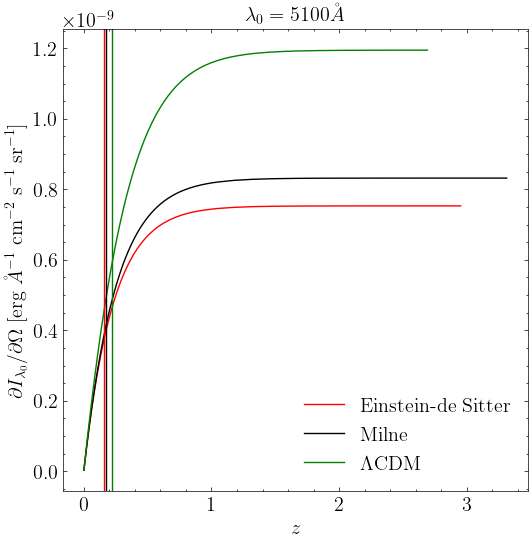
\includegraphics[width=\textwidth]{flux_univers}
                \caption{Illustration e la méthode de calcul, barres verticales indiquent 
                la position de $z_{\text{median}}$ comme le redshift où l'intensité atteint la 
        moitié de son maximum. L'intégrale est calculé jusqu'à ce qu'un plateau soit atteint.}
                \label{fig:flux}
        \end{subfigure}
        ~
        \begin{subfigure}[t]{0.45\textwidth}
                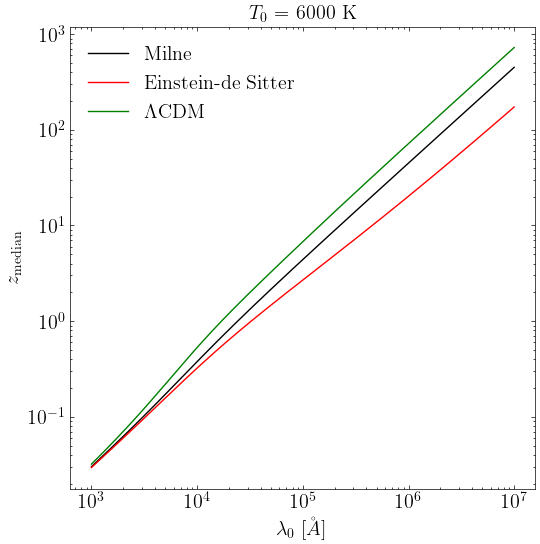
\includegraphics[width=\linewidth]{z_median_univers}
                \caption{Redshift median attendu dans un interval du spectre 
                électromagnétique.}
                \label{fig:z_median}
        \end{subfigure}
\end{figure}

On a utilisé les résultats de la collaboration Planck pour l'univers $\Lambda$CDM:
\begin{table}[H]
        \centering
        \begin{tabular}{cc}
                \toprule
                $h$ & 0.676 \\
                $\Omega_{0m}$ & 0.309\\
                $\Omega_{0r}$ & 0 \\
                $\Omega_{0\Lambda}$ & 0.679\\
                \bottomrule
                
        \end{tabular}
        \caption{Paramètres de $\Lambda$CDM}
        \label{tab:LCDMparam}
\end{table}
On a aussi définit les paramètres physique suivants (\cite{Wesson1991}):
\begin{table}[H]
        \centering
        \begin{tabular}{cc}
                \toprule 
                $T_0$ & $6000\, \text{K}$ \\
                $\epsilon_0 $ & $2.5 h\times 10^{8}\, L_{\odot}\, \text{Mpc}^{-3}$ \\
                $\lambda_0$ & $5100\s \angstrom$ \\
                \bottomrule 
        \end{tabular}
        \caption{Paramètres physiques, où $\epsilon_0 = n_0L_0$ est la densité 
        d'énergie lumineuse.}
        \label{tab:PhysParam}
\end{table}
%L'approximation $w\simeq 0$ (équation d'état) est assez bonne pour les résultats de Planck.

\subsection{Discussion}





\section{Homogénéité de l'Univers}
On considère un échantillon de galaxies du sondage BOSS  dans un cône:
\begin{enumerate}
        \item $0.001 \leq z \leq 0.4$
        \item $156^{\circ} \leq \text{ra} \leq 160^{\circ}$
        \item $27^{\circ} \leq \text{dec} \leq 33^{\circ}$
\end{enumerate}
Notre échantillon contient $N_\text{gal} = ?$ galaxies


\subsection{Nombre de voisins dans une sphère de rayon $r$}
Une première approche pour modéliser l'excès de la densité numérique par rapport à 
un processus de Poisson est de moyenner le nombre de voisins d'une galaxie dans une 
sphère de rayon $r$. Le comportement attendu est que le nombre de galaxie augmente selon 
$r^3$ pour un processus de Poisson. Ainsi, une mesure d'homogénéité est 
\[
        \eta(< r) + 1 = \frac{\langle N_{\text{échantillon}}(<r)\rangle}{
        \langle N_{\text{synthétique}}(<r)\rangle}
\]
où $N_{\text{synthétique}}(<r)$ est le nombre de voisins dans un catalogue synthétique 
avec une distribution de densité uniforme. $\eta(<r) \rightarrow 0$ lorsque la distribution 
devient homogène à l'échelle sondée. La moyenne est pesée pour tenir compte du bruit de 
Poisson.
%En principe, la densité devrait converger vers la densité 
%moyenne de l'échantillon $\bar{n}$ lorsque l'échelle $r$ est suffisamment grande pour que les 
%effets d'agglomérations aux plus petites échelles soient marginalisés dans la moyenne. 
%Autrement dit, la résolution diminue aux grandes échelles et 
%les points à l'intérieur d'une agglomération se confondent. La distribution de densité 
%des agglomération 
%est quant à elle uniforme, d'où le processus de Poisson.


\subsection{Fonction d'autocovariance $\xi(r)$}

On définit la fonction d'autocovariance $\xi(r)$ comme l'amplitude de la tendance 
aux galaxies de s'agglomérer:
\[
        dP = \bar{n} (1 + \xi(r)) dV
\]
où $dP$ mesure la probabilité de trouvé un voisin à une distance $r$ dans un un volume $dV$. 
Ainsi, $\xi(r)$ mesure l'excès de probabilité par rapport à un processus de Poisson (où 
la probabilité est fixe $dP^{\text{Poisson}} = \bar{n}dV$). 




\section{Les unités en cosmologie}
On considère les unités naturelles
\[
        c = \hbar = k_B = 1
\]
Dans ce système d'unité, le temps et les distances sont en cm, de même que l'inverse de la masse $\text{m}^{-1}$, 
et l'inverse de l'énergie $\text{E}^{-1}$. On trouve les facteurs de conversions suivants
\begin{align*}
        1\, \text{s} &\mapsto  29,979,245,800 \,\, \text{cm} \\
        1\, \si{\electronvolt^{-1}} &\mapsto \frac{\hbar c }{\si{\electronvolt}}= 1.973 \times 10^{-5} \,\, \text{cm} \\
        1\, \text{g}^{-1} &\mapsto \frac{\hbar}{c} \text{g}^{-1} = 3.518 \times 10^{-38} \,\, \text{cm}   
\end{align*}
\subsection{$H_0$}
\[
        H_0 \equiv 100 h \s \si{\kilo\meter \per \second \per \mega \parsec}
\]
\subsubsection{Conversion en $\si{\electronvolt}$}
\[
        H_0 \mapsto \hbar H_0 \simeq 2.13h \times 10^{-33}\,\, \si{\electronvolt}
\]

\subsubsection{Conversion en $\textmd{Mpc}^{-1}$}\label{sec:TailleUnivers}
\[
        H_0 \mapsto \frac{H_0}{c} \simeq 3.34h \times 10^{-4} \,\, \text{Mpc}^{-1}
\]
\subsubsection{Conversion en $\textmd{Gyr}^{-1}$}
\[
        H_0 \simeq 0.10h \,\, \text{Gyr}^{-1}
\]

\subsubsection{Conversion en $\textmd{m}\, \textmd{s}^{-2}$}
\[
        H_0 \mapsto H_0 c \simeq 9.72h \times 10^{-10}\,\, \text{m}\,\,\text{s}^{-2}
\]

\subsection{Taille caractéristique}
L'Univers devient homogène à la distance caractéristique où l'accélération gravitationnelle de Newton 
d'un amas de galaxie (typiquement $10^{15} M_\odot$) 
est égale au taux d'expansion de l'univers au temps présent. 
\[
        \frac{GM}{R^2} = H_0 c \implies R = \sqrt{\frac{GM}{H_0 c}} \simeq 37.9h^{-1/2} \,\, \text{Mpc}
\]

\subsection{$\rho_{\textmd{crit}}$}
La densité critique est
\[
        \rho_{\text{crit}} = \frac{3 H_0^2}{8 \pi G}
\]

\subsubsection{Conversion en $\si{\gram \per\centi\meter^{3}}$}
\[
        \rho_{\text{crit}} = 1.88h^{2} \times 10^{-29}\,\, \text{g} \,\, \text{cm}^{-3}
\]

\subsubsection{Conversion en $\si{\giga \electronvolt^{4}}$}
\[
        \rho_{\text{crit}} \mapsto \frac{c}{\hbar} (\hbar c)^4 \rho_{\text{crit}}
        \simeq 8.096 h^2 \times 10^{-47}\,\, \si{\giga\electronvolt^{4}}
\]

\subsubsection{Conversion en $\si{\electronvolt \per \centi\meter^{3}}$}
\[
        \rho_{\text{crit}} \mapsto c^2 \rho_{\text{crit}} \simeq 1.05 h^2 \times 10^{4}\,\, 
        \si{\electronvolt}\, \text{cm}^{-3}
\]

\subsubsection{Conversion en \textmd{protons}/$\textmd{cm}^{3}$}
\[
        \rho_{\text{crit}} \mapsto \frac{\rho_{\text{crit}}}{m_p} \simeq 
        1.123h^2\times 10^{-5}\,\, \text{protons}\,\,\text{cm}^{-3}
\]

\subsubsection{Conversion en $M_\odot / \textmd{Mpc}^{3}$}
\[
        \rho_{\text{crit}} = 2.78h^2 \times 10^{11}\,\, M_\odot\,\, \text{Mpc}^{-3}
\]


\section{Le rayon de Schwarzschild}
Pour estimer la masse de l'Univers, on utilise la densité critique $\rho_{\text{crit}}$ 
et le rayon de Hubble (distance par rapport à l'observateur à partir de laquelle 
la vitesse de récession dépasse la vitesse de la lumière -- aussi nommé horizon cosmique)
\[
        R_H \equiv \frac{c}{H_0} \simeq 2998h^{-1}\,\, \text{Mpc}
\]
%On peut estimer la masse de l'univers en utilisant la fraction de masse 

\[
        M =  \rho_{\text{crit}} \frac{4 \pi R_H^{3}}{3} = \frac{c^3}{2GH_0} 
       \simeq 3.132  h^{-1} \times 10^{22}\, M_\odot
\]
C'est la formule de Hoyle-Carvalho.
Le rayon de Schwarzschild est donc:
\[
        r_s \equiv \frac{2 G M}{c^2} =  R_H
\]
%\[
        %r_{\text{s}} \equiv \frac{2GM}{c^2} \simeq
%\]
%Pour être cohérent , nous devons toutefois utiliser la métrique de Schwarzschild. Ainsi,
%\[
        %R_H^{\text{Sc}} = \int_0^{R_H} \frac{ds}{1 - }
%\]
%Pour calculer le rayon de Schwarzschild de l'Univers visible, on doit d'abord estimer la masse 
%de l'Univers visible. Le paramètre de Hubble nous donne un estimé de la taille de l'Univers. 
%On peut estimer l'horizon comobile (distance hypothétiquement voyagé par un rayon 
%lumineux depuis le début de l'Univers) en utilisant la constante de Hubble mesurée aujourd'hui
%\[
        %\xi = \int_{t_i}^{t_0} c \frac{dt'}{a(t')}
%\]


\section{La métrique}
\subsection{Redéfinir $\pi$}
Existe-t-il un univers où le ratio entre le rayon et la circonférence est constant et 
égal à 3? Pour répondre à la question, on considère un univers homogène et 
isotropique définit par la métrique suivante: 
\[
        ds^2 = \frac{dr^2}{1 - kr^2} + r^2d\Omega^2
\]
où $k \in \{-1, 0, 1\}$ et $r \in [0,1[$ est une coordonnée affine. 
La circonférence d'un cercle est défini par
\[
        C = \oint_\gamma \sqrt{ds^2} = 2 \pi R
\]
où $\gamma$ est la trajectoire avec $r=R$, $\theta=\pi/2$ et 
$\phi \in [0, 2 \pi]$. Le 
rayon du cercle, quant à lui, est définit comme
\[
        R_c = \int_0^R \frac{dr'}{\sqrt{1 - kr'^2}}
\]
Ainsi, on obtient les trois ratio suivant (pour les différentes valeurs de $k$):
\[
        \frac{C}{R_c} = \left\{ 
\begin{matrix}
        2 \pi, & k = 0 \\[3ex]
        \dfrac{2\pi R}{\arcsin R} < 2 \pi, & k = 1 \\[3ex]
        \dfrac{2 \pi R}{\sinh^{-1} R} > 2 \pi, & k = -1

\end{matrix}
        \right.
\]
Pour un espace fermé ($k=1$), le rapport entre la circonférence et le rayon varie 
en fonction de la coordonnée affine du rayon. Dans ce cas, il serait possible de 
redéfinir $\pi = 3$. Examinons l'expansion de Taylor de l'expression pour $k=1$ autour 
de $R = 0$:
\[
        \frac{C}{R_c} \simeq \frac{2 \pi R}{R + \dfrac{R^3}{6} + \mathcal{O}(R^5)}
        \simeq 2 \pi \left(  1 - \frac{R^2}{6} - \mathcal{O}(R^4)\right)
\]
Pour redéfinir $\pi = 3$, alors le cercle de référence 
doit être crée à la coordonnée affine
\[
        R^* \simeq 0.532
\]
Dans la perspective de cet univers, le rapport circonférence sur le rayon suit la loi
\[
        \frac{C}{R_c} \simeq 6 \left( 1 - \frac{(R - R^*)^3}{6|R - R^{*}|} -
                \mathcal{O}\left(\frac{(R - R^{*})^{5}}{|R - R^{*}|}\right) \right),
\]

Donc, la réponse est oui, il est parfaitement légitime de redéfinir $\pi = 3$ dans un 
univers fermé (de courbure positive) en utilisant un cercle de référence avec un rayon 
de coordonnée affine $R^{*} \simeq 0.532$.

Toutefois, \textbf{il n'existe pas d'univers où le ratio circonférence sur rayon est constant 
où} $\pi \not= 3.14159...$. Le ratio est constant seulement dans un univers Euclidien où 
$\pi$ ne peut pas prendre une valeur différente de celle connue. C'est à dire que 
\[
        \pi \equiv \frac{1}{2}\int_{-1}^1 \frac{d\xi}{\sqrt{1 - \xi^2}}
\]
qui est basé sur la métrique $ds^2 = dx^2 + dy^2$ 
avec la condition $x^2 + y^2 = 1$. En ce sens, la valeur de la constante $\pi$ ne peut pas être 
changé en ce sens qu'elle est une construction théorique liée à un espace Euclidien.

\subsection{\textit{Hartle}, exercice 2, ch. 2}
Supposant que l'on puisse se situer sur la surface du Soleil et qu'on répéter l'expérience 
de Gauss pour mesurer les angles d'un triangle. La différence entre la somme des angles 
mesurées $\sum \alpha_i$ et la somme attendu pour un espace Euclidien $\pi$ est 
\[
        \sum \alpha_i - \pi \simeq \frac{A_{\triangle}}{R_\odot^{2}} 
        \left( \frac{GM_\odot}{R_\odot c^2} \right)
\]
Le premier facteur est un effet purement géométrique (le Soleil est une sphère en première 
approximation), alors que le second facteur est une correction approtée par la relativité générale.

En supposant qu'on répète l'expérience de Gauss, on mesure l'angle du triangle entre les monts 
Brocken, Hohenhagen et Inselberg. Les distances entre ces montagnes sont $69\, \text{km}$, 
$85\, \text{km}$ et $107\, \text{km}$. En utilisant la formule de Héron, 
\[
        A_\triangle \simeq 2929\, \text{km}^2
\]
De sortes que
\[
        \frac{A_\triangle}{R^2} \simeq 
\left\{ 
\begin{matrix}
        6.05 \times 10^{-9}, & R_\odot \\
        7.20 \times 10^{-5}, & R_\oplus
\end{matrix}
\right.
\]
et
\[
        \frac{GM_\odot}{c^2R_\odot} \simeq 
\left\{ 
\begin{matrix}
        2.12 \times 10^{-6}, & R_\odot \\
        6.95 \times 10^{-10}, & R_\oplus
\end{matrix}
\right.
\]
Pour une déviation égale à
\[
        \sum \alpha_i - \pi \simeq 
\left\{ 
\begin{matrix}
        1.29 \times 10^{-14}, & R_\odot \\ 
        5.01 \times 10^{-14}, & R_\oplus
\end{matrix}
\right.
\]
On remarque que dans les deux cas, la déviation est similaire mais la source de cette déviation 
est différente. Pour le Soleil, l'effet gravitationnel est beaucoup plus important que l'effet géométrique.


%\bliography{../bibfile}
\bibliography{bibfile.bib}
\bibliographystyle{plain}

%\begin{thebibliography}{9}
        %\bibitem{StabellRefsdal}
        %Stabell, R., \& Refsdal, S. (1966). Classification of General Relativistic World Models. Monthly Notices of the Royal Astronomical Society, 132(2), 379–388. \url{https://doi.org/10.1093/mnras/132.2.379}
        %\bibitem{Wesson91}
        %Wesson, P. S. (1991). Olbers’s paradox and theectral intensity of the extragalactic background light. In The Astrophysical Journal (Vol. 367). \url{https://doi.org/10.1086/169638}

        %\bibitem{Wesson87}
        %Wesson, P. S., Valle, K., \& Stabell, R. (1987). The extragalactic background light and a definitive resolution of Olbers’s paradox. The Astrophysical Journal, 317, 601. \url{https://doi.org/10.1086/165306}
        
%\end{thebibliography}

\end{document}

